\documentclass[pmlr]{jmlr}% new name PMLR (Proceedings of Machine Learning Research)

 % The following packages will be automatically loaded:
 % amsmath, amssymb, natbib, graphicx, url, algorithm2e

 %\usepackage{rotating}% for sideways figures and tables
\usepackage{longtable}% for long tables

 % The booktabs package is used by this sample document
 % (it provides \toprule, \midrule and \bottomrule).
 % Remove the next line if you don't require it.
\usepackage{booktabs}
 % The siunitx package is used by this sample document
 % to align numbers in a column by their decimal point.
 % Remove the next line if you don't require it.
\usepackage[load-configurations=version-1]{siunitx} % newer version
 %\usepackage{siunitx}

 % The following command is just for this sample document:
\newcommand{\cs}[1]{\texttt{\char`\\#1}}

 % Define an unnumbered theorem just for this sample document:
\theorembodyfont{\upshape}
\theoremheaderfont{\scshape}
\theorempostheader{:}
\theoremsep{\newline}
\newtheorem*{note}{Note}

 % change the arguments, as appropriate, in the following:
\jmlrvolume{1}
\jmlryear{2010}
\jmlrworkshop{Workshop Title}

\title[SLAPI]{Simultaneous Localization and Active Phenomenon Inference (SLAPI)}

 % Use \Name{Author Name} to specify the name.

 % Spaces are used to separate forenames from the surname so that
 % the surnames can be picked up for the page header and copyright footer.
 
 % If the surname contains spaces, enclose the surname
 % in braces, e.g. \Name{John {Smith Jones}} similarly
 % if the name has a "von" part, e.g \Name{Jane {de Winter}}.
 % If the first letter in the forenames is a diacritic
 % enclose the diacritic in braces, e.g. \Name{{\'E}louise Smith}

 % *** Make sure there's no spurious space before \nametag ***

 % Two authors with the same address
  \author{\Name{Olivier L. Georgeon} \Email{ogeorgeon@univ-catholyon.fr}\\
  \addr UR Confluence, Sciences et Humanités (EA 1598) - Lyon Catholic University, France\\
   \Name{Titouan Knockaert} \Email{titouan.knockaert@gmail.com}\\
  \addr Université Claude Bernard Lyon 1, LIRIS CNRS UMR5205, F-69622 Villeurbanne, France
}

 % Three or more authors with the same address:
 % \author{\Name{Author Name1} \Email{an1@sample.com}\\
 %  \Name{Author Name2} \Email{an2@sample.com}\\
 %  \Name{Author Name3} \Email{an3@sample.com}\\
 %  \Name{Author Name4} \Email{an4@sample.com}\\
 %  \Name{Author Name5} \Email{an5@sample.com}\\
 %  \Name{Author Name6} \Email{an6@sample.com}\\
 %  \Name{Author Name7} \Email{an7@sample.com}\\
 %  \Name{Author Name8} \Email{an8@sample.com}\\
 %  \Name{Author Name9} \Email{an9@sample.com}\\
 %  \Name{Author Name10} \Email{an10@sample.com}\\
 %  \Name{Author Name11} \Email{an11@sample.com}\\
 %  \Name{Author Name12} \Email{an12@sample.com}\\
 %  \Name{Author Name13} \Email{an13@sample.com}\\
 %  \Name{Author Name14} \Email{an14@sample.com}\\
 %  \addr Address}


 % Authors with different addresses:
 % \author{\Name{Author Name1} \Email{abc@sample.com}\\
 % \addr Address 1
 % \AND
 % \Name{Author Name2} \Email{xyz@sample.com}\\
 % \addr Address 2
 %}

\editor{Editor's name}
 % \editors{List of editors' names}

\begin{document}

\maketitle

\begin{abstract}
This is the abstract for this article.
\end{abstract}
\begin{keywords}
List of keywords
\end{keywords}

\section{Introduction}
\label{sec:intro}

The problem of getting mobile robots to autonomously learn the position of surrounding objects, recognize them, and keep track of their relative displacements is considered by many to be a key prerequisite of truly autonomous robots. 
Within this framework, the SLAM problem (Simultaneous Localization and Mapping) has been formalized and studied since the 1990s: constructing and updating a map of an unknown environment while simultaneously keeping track of the robot's position within it.
SLAM algorithms are tailored to the available resources: odometric sensors, sensors of the environment, computational capacities, as well as the landmarks' properties, quantity, and dynamics, and the usage intended for the robot.
When displacements are imprecise and odometric data is not available, when landmarks are not directly identifiable, and below a certain level of scarcity and noise in the sensory data relative to the environment’s complexity, it becomes difficult to perform SLAM accurately enough to use the robot for tasks involving complex navigation. 
For such robots, we propose the SLAPI problem:  Simultaneous Localization and Active Phenomenon Inference.
In contrast with SLAM, SLAPI does not aim at constructing a map to use for navigation. 
Instead, it aims at organizing behavior spatially in the vicinity of objects to design robots that exhibit intrinsic motivation such as playfulness and curiosity as they discover and interact with unknown objects. 
Possible applications may not include delivery tasks but may include entertainment and games, similar to playing with pets. 
SLAPI makes no assumption that landmarks can be directly and passively uniquely identified through sensors. 
The robot must rather actively interact with objects, possibly from different angles and through different modalities of control loops, to categorize and recognize objects, and possibly use them as landmarks. 
This process is called active phenomenon inference. 
Here the term phenomenon refers to the knowledge of physical objects actively constructed by the robot from its point of view and "as the robot experiences the object through interaction". 
We designed a proof-of-concept algorithm to illustrate the SLAPI problem. 
We demonstrated it in a robot mounted on omnidirectional wheels and endowed with an echo-localization sensor, photosensitive sensors, and an inertial measurement unit, but no camera and lidar. 
As the robot circles around an object, it constructs the phenomenon corresponding to this object under the form of the set of the spatially-localized control loops that the object affords to the robot. 
New elements can be subsequently added to this set as the robot improves its knowledge of the object. 
Results show that the robot drew out a few cries of amusement and endearment from some human observers, which encourages us to keep improving this range of algorithms. 
Moreover, we believe that the study of SLAPI problems can shed some light on how animals construct knowledge of objects through sensorimotor interactions, while keeping this knowledge grounded in experience. 
It can also provide an angle of attack to the more general AI problem of self-motivated open-ended learning in the real world.

\begin{note}
This is an numbered theorem-like environment that was defined in
this document's preamble.
\end{note}

\subsection{Sub-sections}

Sub-sections are produced using \verb|\subsection|.

\subsubsection{Sub-sub-sections}

Sub-sub-sections are produced using \verb|\subsubsection|.

\paragraph{Sub-sub-sub-sections}

Sub-sub-sub-sections are produced using \verb|\paragraph|.
These are unnumbered with a running head.

\subparagraph{Sub-sub-sub-sub-sections}

Sub-sub-sub-sub-sections are produced using \verb|\subparagraph|.
These are unnumbered with a running head.

\section{Cross-Referencing}

Always use \verb|\label| and \verb|\ref| (or one of the commands
described below) when cross-referencing.  For example, the next
section is Section~\ref{sec:math}. The \textsf{jmlr} class
provides some convenient cross-referencing commands:
\verb|\sectionref|, \verb|\equationref|, \verb|\tableref|,
\verb|\figureref|, \verb|\algorithmref|, \verb|\theoremref|,
\verb|\lemmaref|, \verb|\remarkref|, \verb|\corollaryref|,
\verb|\definitionref|, \verb|\conjectureref|, \verb|\axiomref|,
\verb|\exampleref| and \verb|\appendixref|. The argument of these
commands may either be a single label or a comma-separated list
of labels. Examples:

Referencing sections: \sectionref{sec:math} or
\sectionref{sec:intro,sec:math} or
\sectionref{sec:intro,sec:math,sec:tables,sec:figures}.

Referencing equations: \equationref{eq:trigrule} or
\equationref{eq:trigrule,eq:df} or
\equationref{eq:trigrule,eq:f,eq:df,eq:y}.

Referencing tables: \tableref{tab:operatornames} or
\tableref{tab:operatornames,tab:example} or
\tableref{tab:operatornames,tab:example,tab:example-booktabs}.

Referencing figures: \figureref{fig:image} or
\figureref{fig:image,fig:teximage} or
\figureref{fig:image,fig:teximage,fig:subfigex} or
\figureref{fig:image-a,fig:image-b}.

Referencing algorithms: \algorithmref{alg:gauss} or
\algorithmref{alg:gauss,alg:moore} or
\algorithmref{alg:gauss,alg:moore,alg:net}.

Referencing theorem-like environments: \theoremref{thm:eigenpow},
\lemmaref{lem:sample}, \remarkref{rem:sample}, 
\corollaryref{cor:sample}, \definitionref{def:sample},
\conjectureref{con:sample}, \axiomref{ax:sample} and
\exampleref{ex:sample}.

Referencing appendices: \appendixref{apd:first} or
\appendixref{apd:first,apd:second}.

\section{Equations}
\label{sec:math}

The \textsf{jmlr} class loads the \textsf{amsmath} package, so
you can use any of the commands and environments defined there.
(See the \textsf{amsmath} documentation for further
details.\footnote{Either \texttt{texdoc amsmath} or
\url{http://www.ctan.org/pkg/amsmath}})

Unnumbered single-lined equations should be displayed using
\verb|\[| and \verb|\]|. For example:
\[E = m c^2\]
Numbered single-line equations should be displayed using the
\texttt{equation} environment. For example:
\begin{equation}\label{eq:trigrule}
\cos^2\theta + \sin^2\theta \equiv 1
\end{equation}
This can be referenced using \verb|\label| and \verb|\equationref|.
For example, \equationref{eq:trigrule}.

Multi-lined numbered equations should be displayed using the
\texttt{align} environment.\footnote{For reasons why you 
shouldn't use the obsolete \texttt{eqnarray} environment, see
Lars Madsen, \emph{Avoid eqnarray!} TUGboat 33(1):21--25, 2012.} For example:
\begin{align}
f(x) &= x^2 + x\label{eq:f}\\
f'(x) &= 2x + 1\label{eq:df}
\end{align}
Unnumbered multi-lined equations should be displayed using the
\texttt{align*} environment. For example:
\begin{align*}
f(x) &= (x+1)(x-1)\\
&= x^2 - 1
\end{align*}
If you want to mix numbered with unnumbered lines use the
align environment and suppress unwanted line numbers with
\verb|\nonumber|. For example:
\begin{align}
y &= x^2 + 3x - 2x + 1\nonumber\\
&= x^2 + x + 1\label{eq:y}
\end{align}
An equation that is too long to fit on a single line can be
displayed using the \texttt{split} environment. 
Text can be embedded in an equation using \verb|\text| or
\verb|\intertext| (as used in \theoremref{thm:eigenpow}).
See the \textsf{amsmath} documentation for further details.

\subsection{Operator Names}
\label{sec:op}

Predefined operator names are listed in \tableref{tab:operatornames}.
For additional operators, either use \verb|\operatorname|,
for example $\operatorname{var}(X)$ or declare it with
\verb|\DeclareMathOperator|, for example
\begin{verbatim}
\DeclareMathOperator{\var}{var}
\end{verbatim}
and then use this new command. If you want limits that go above and
below the operator (like \verb|\sum|) use the starred versions
(\verb|\operatorname*| or \verb|\DeclareMathOperator*|).

\begin{table}[htbp]
\floatconts
  {tab:operatornames}%
  {\caption{Predefined Operator Names (taken from 
   \textsf{amsmath} documentation)}}%
  {%
\begin{tabular}{rlrlrlrl}
\cs{arccos} & $\arccos$ &  \cs{deg} & $\deg$ &  \cs{lg} & $\lg$ &  \cs{projlim} & $\projlim$ \\
\cs{arcsin} & $\arcsin$ &  \cs{det} & $\det$ &  \cs{lim} & $\lim$ &  \cs{sec} & $\sec$ \\
\cs{arctan} & $\arctan$ &  \cs{dim} & $\dim$ &  \cs{liminf} & $\liminf$ &  \cs{sin} & $\sin$ \\
\cs{arg} & $\arg$ &  \cs{exp} & $\exp$ &  \cs{limsup} & $\limsup$ &  \cs{sinh} & $\sinh$ \\
\cs{cos} & $\cos$ &  \cs{gcd} & $\gcd$ &  \cs{ln} & $\ln$ &  \cs{sup} & $\sup$ \\
\cs{cosh} & $\cosh$ &  \cs{hom} & $\hom$ &  \cs{log} & $\log$ &  \cs{tan} & $\tan$ \\
\cs{cot} & $\cot$ &  \cs{inf} & $\inf$ &  \cs{max} & $\max$ &  \cs{tanh} & $\tanh$ \\
\cs{coth} & $\coth$ &  \cs{injlim} & $\injlim$ &  \cs{min} & $\min$ \\
\cs{csc} & $\csc$ &  \cs{ker} & $\ker$ &  \cs{Pr} & $\Pr$
\end{tabular}\par
\begin{tabular}{rlrl}
\cs{varlimsup} & $\varlimsup$ 
& \cs{varinjlim} & $\varinjlim$\\
\cs{varliminf} & $\varliminf$ 
& \cs{varprojlim} & $\varprojlim$
\end{tabular}
}
\end{table}

\section{Vectors and Sets}
\label{sec:vec}

Vectors should be typeset using \cs{vec}. For example $\vec{x}$.
The \textsf{jmlr} class also provides \cs{set} to typeset a
set. For example $\set{S}$.

\section{Floats}
\label{sec:floats}

Floats, such as figures, tables and algorithms, are moving
objects and are supposed to float to the nearest convenient
location. Please don't force them to go in a particular place. In
general it's best to use the \texttt{htbp} specifier and don't
put the figure or table in the middle of a paragraph (that is
make sure there's a paragraph break above and below the float).
Floats are supposed to have a little extra space above and below
them to make them stand out from the rest of the text. This extra
spacing is put in automatically and shouldn't need modifying.

To ensure consistency, please \emph{don't} try changing the format of the caption by doing
something like:
\begin{verbatim}
\caption{\textit{A Sample Caption.}}
\end{verbatim}
or
\begin{verbatim}
\caption{\em A Sample Caption.}
\end{verbatim}
You can, of course, change the font for individual words or 
phrases, for example:
\begin{verbatim}
\caption{A Sample Caption With Some \emph{Emphasized Words}.}
\end{verbatim}

\subsection{Tables}
\label{sec:tables}


\begin{table}[htbp]
 % The first argument is the label.
 % The caption goes in the second argument, and the table contents
 % go in the third argument.
\floatconts
  {tab:actions}%
  {\caption{Data exchanged between the PC and the robot through wifi}}%
  {\begin{tabular}{l|l}
  \toprule
  PC to Robot & Action code, focus position (x, y), estimated speed (x,y)\\
  \midrule
  Robot to PC & Outcome code, echo distance, head direction, yaw, azimuth, duration\\
  \bottomrule
  \end{tabular}}
\end{table}

\begin{table}[htbp]
	\floatconts
	{tab:subtabex}
	{\caption{Actions available to the robot and their possible outcomes}}
	{%
		\subtable[Actions]{%
			\label{tab:ab}%
			\begin{tabular}{lc}
				\toprule
				\bfseries Action & \bfseries Span\\
				\midrule
				Forward & During 1 second\\
				Backward & or until line\\
				Shift left & detection\\
				Shift right & \\ \hline
				Turn left & $\pi/4$ \\
				Turn right & $-\pi/4$ \\ \hline
				Head scan & $[-\pi/2, \pi/2]$ \\
				\bottomrule
		\end{tabular}}
		\qquad
		\subtable[Outcomes]{%
			\label{tab:cd}%
			\begin{tabular}{lc}
				\toprule
				\bfseries Outcome & \bfseries Description\\
				\midrule
				Line left & Floor sensors cross \\
				Line front & luminosity threshold\\
				Line right & \\ \hline
				Echo lost focus & No echo where expected \\ \hline
				Echo left & Direction\\  
				Echo right & and range \\  
				Echo far left & of the \\  
				Echo far right & nearest echo\\  
				Echo far front & \\
				Echo close front & \\ \hline
				Default & No line, no echo \\ 
				\bottomrule
			\end{tabular}
		}
	}
\end{table}


\subsection{Figures}
\label{sec:figures}

Figures should go in the \texttt{figure} environment. Within this
environment, use \verb|\floatconts| to correctly position the
caption and center the image. Use \verb|\includegraphics|
for external graphics files but omit the file extension. Do not
use \verb|\epsfig| or \verb|\psfig|. If you want to scale the
image, it's better to use a fraction of the line width rather
than an explicit length. For example, see \figureref{fig:image}.

\begin{figure}[htbp]
 % Caption and label go in the first argument and the figure contents
 % go in the second argument
  \floatconts
  {fig:robot}
  {\caption{The interaction cycle}}
  {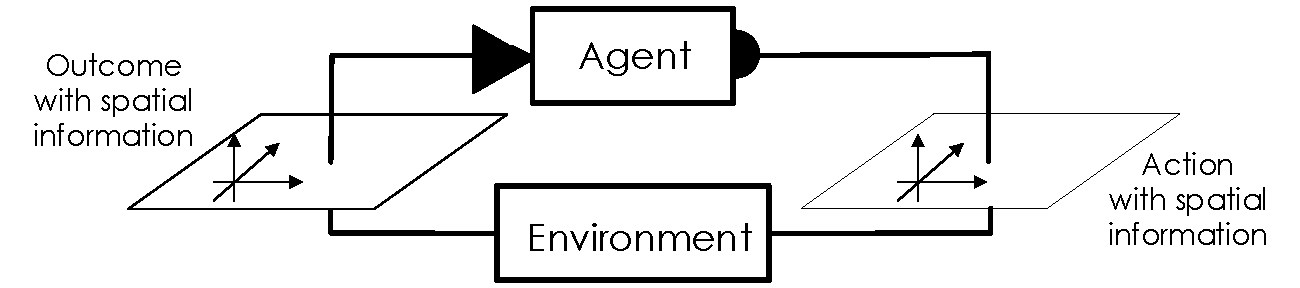
\includegraphics[width=0.8\linewidth]{images/Figure_0_Cycle}}
\end{figure}

\begin{figure}[htbp]
	% Caption and label go in the first argument and the figure contents
	% go in the second argument
	\floatconts
	{fig:robot}
	{\caption{The robot}}
	{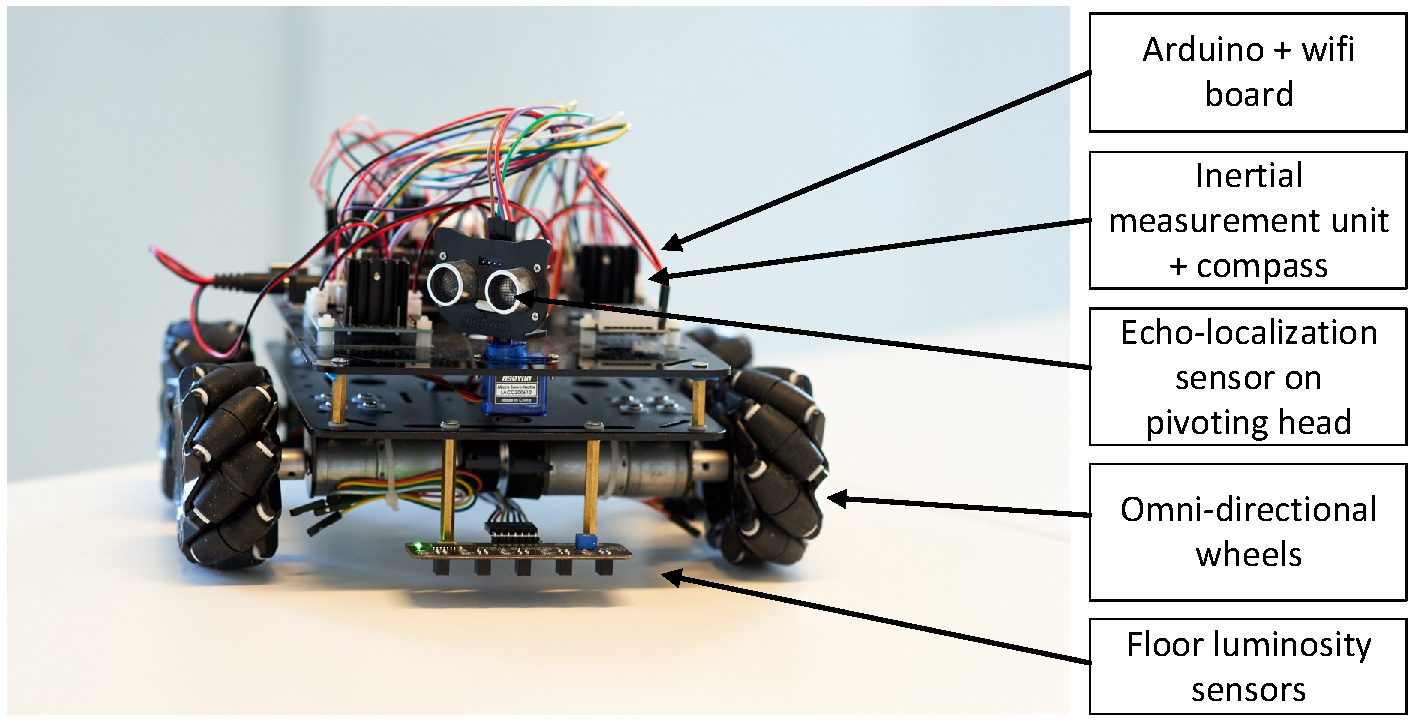
\includegraphics[width=0.8\linewidth]{images/Figure_1_Robot}}
\end{figure}


\begin{figure}[htbp]
	% Caption and label go in the first argument and the figure contents
	% go in the second argument
	\floatconts
	{fig:architecture}
	{\caption{The Model-View-Controller architecture}}
	{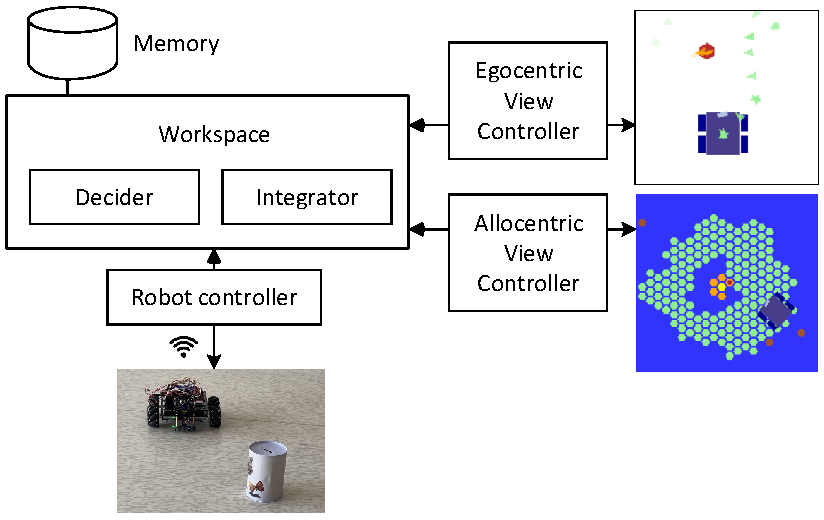
\includegraphics[width=0.8\linewidth]{images/Figure_2_Architecture}}
\end{figure}


If your image is made up of \LaTeX\ code (for example, commands
provided by the \textsf{pgf} package) you can include it using
\cs{includeteximage} (defined by the \textsf{jmlr} class). This
can be scaled and rotated in the same way as \cs{includegraphics}.
For example, see \figureref{fig:teximage}.

\begin{figure}[htbp]
\floatconts
  {fig:teximage}
  {\caption{The robot}}
  {\includeteximage[angle=45]{images/Figure_1_Robot}}
\end{figure}

If the figure is too wide to fit on the page, you can use the
\texttt{sidewaysfigure} environment defined in the
\textsf{rotating} package.

It's best not to use \verb|\graphicspath| with the \textsf{jmlr} class
as it can cause problems with the production editing process. If the
images are contained in a subdirectory, specify this when you
include the image, for example \verb|\includegraphics{figures/mypic}|.

\subsection{Sub-Figures}
\label{sec:subfigures}

Sub-figures can be created using \verb|\subfigure|, which is
defined by the \textsf{jmlr} class. The optional argument allows
you to provide a subcaption. The label should be placed in the
mandatory argument of \verb|\subfigure|. You can reference the
entire figure, for example \figureref{fig:subfigex}, or you can
reference part of the figure using \verb|\figureref|, for example
\figureref{fig:image-a}. Alternatively you can reference the
subfigure using \verb|\subfigref|, for example
\subfigref{fig:image-a,fig:image-b} in \figureref{fig:subfigex}.

\begin{figure}[htbp]
\floatconts
  {fig:subfigex}
  {\caption{An Example With Sub-Figures.}}
  {%
    \subfigure[Image A]{\label{fig:image-a}%
      \includegraphics[width=0.2\linewidth]{example-image-a}}%
    \qquad
    \subfigure[Image B]{\label{fig:image-b}%
      \includegraphics[width=0.25\linewidth]{example-image-b}}
  }
\end{figure}

By default, the sub-figures are aligned on the baseline.
This can be changed using the second optional argument
of \verb|\subfigure|. This may be \texttt{t} (top), \texttt{c}
(centered) or \texttt{b} (bottom). For example, the subfigures
\subfigref{fig:image-a2,fig:image-b2} in \figureref{fig:subfigex2}
both have \verb|[c]| as the second optional argument.

\begin{figure}[htbp]
\floatconts
  {fig:subfigex2}
  {\caption{Another Example With Sub-Figures (with a Cramped
    Sub-Caption).}}
  {%
    \subfigure[Image A][c]{\label{fig:image-a2}%
      \includegraphics[width=0.1\linewidth]{example-image-a}}%
    \qquad
    \subfigure[Image B][c]{\label{fig:image-b2}%
      \includegraphics[width=0.3\linewidth]{example-image-b}}
  }%
\end{figure}

Note that a very narrow sub-float will leave little space for the
sub-caption, which will likely cause Underfull/Overfull hbox warnings.

You can set the length \verb|\jmlrminsubcaptionwidth| to indicate
the minimum width to be made available for the sub-captions, as in
\figureref{fig:subfigex3}.

\begin{figure}[htbp]
\floatconts
  {fig:subfigex3}
  {\caption{Another Example With Sub-Figures (with a Less Cramped
    Sub-Caption).}}
  {\setlength{\jmlrminsubcaptionwidth}{0.2\linewidth}%
    \subfigure[Image A][c]{\label{fig:image-a3}%
     \includegraphics[width=0.1\linewidth]{example-image-a}}%
    \qquad
    \subfigure[Image B][c]{\label{fig:image-b3}%
      \includegraphics[width=0.2\linewidth]{example-image-b}}
  }%
\end{figure}


\subsection{Algorithms}
\label{sec:algorithms}

Enumerated textual algorithms can be displayed using the
\texttt{algorithm} environment. Within this environment, use
use an \texttt{enumerate} or nested \texttt{enumerate} environments.
For example, see \algorithmref{alg:gauss}. Note that algorithms
float like figures and tables.

\begin{algorithm}[htbp]
\floatconts
{alg:gauss}% label
{\caption{The Gauss-Seidel Algorithm}}
{% contents
\begin{enumerate}
  \item For $k=1$ to maximum number of iterations
    \begin{enumerate}
      \item For $i=1$ to $n$
        \begin{enumerate}
        \item $x_i^{(k)} = 
          \frac{b_i - \sum_{j=1}^{i-1}a_{ij}x_j^{(k)}
          - \sum_{j=i+1}^{n}a_{ij}x_j^{(k-1)}}{a_{ii}}$
        \item If $\|\vec{x}^{(k)}-\vec{x}^{(k-1)} < \epsilon\|$,
          where $\epsilon$ is a specified stopping criteria, stop.
      \end{enumerate}
    \end{enumerate}
\end{enumerate}
}
\end{algorithm}

If you'd rather have the same numbering throughout the algorithm
but still want the convenient indentation of nested 
\texttt{enumerate} environments, you can use the
\texttt{enumerate*} environment provided by the \textsf{jmlr}
class. For example, see \algorithmref{alg:moore}.

\begin{algorithm}
\floatconts
{alg:moore}% label
{\caption{Moore's Shortest Path}}%caption
{% main float content
Given a connected graph $G$, where the length of each edge is 1:
\begin{enumerate*}
  \item Set the label of vertex $s$ to 0
  \item Set $i=0$
  \begin{enumerate*}
    \item \label{step:locate}Locate all unlabelled vertices 
          adjacent to a vertex labelled $i$ and label them $i+1$
    \item If vertex $t$ has been labelled,
    \begin{enumerate*}
      \item[] the shortest path can be found by backtracking, and 
      the length is given by the label of $t$.
    \end{enumerate*}
    otherwise
    \begin{enumerate*}
      \item[] increment $i$ and return to step~\ref{step:locate}
    \end{enumerate*}
  \end{enumerate*}
\end{enumerate*}
}
\end{algorithm}

Pseudo code can be displayed using the \texttt{algorithm2e}
environment. This is defined by the \textsf{algorithm2e} package
(which is automatically loaded) so check the \textsf{algorithm2e}
documentation for further details.\footnote{Either \texttt{texdoc
algorithm2e} or \url{http://www.ctan.org/pkg/algorithm2e}}
For an example, see \algorithmref{alg:net}.

\begin{algorithm2e}
\caption{Computing Net Activation}
\label{alg:net}
 % older versions of algorithm2e have \dontprintsemicolon instead
 % of the following:
 %\DontPrintSemicolon
 % older versions of algorithm2e have \linesnumbered instead of the
 % following:
 %\LinesNumbered
\KwIn{$x_1, \ldots, x_n, w_1, \ldots, w_n$}
\KwOut{$y$, the net activation}
$y\leftarrow 0$\;
\For{$i\leftarrow 1$ \KwTo $n$}{
  $y \leftarrow y + w_i*x_i$\;
}
\end{algorithm2e}

\section{Description Lists}

The \textsf{jmlr} class also provides a description-like 
environment called \texttt{altdescription}. This has an
argument that should be the widest label in the list. Compare:
\begin{description}
\item[add] A method that adds two variables.
\item[differentiate] A method that differentiates a function.
\end{description}
with
\begin{altdescription}{differentiate}
\item[add] A method that adds two variables.
\item[differentiate] A method that differentiates a function.
\end{altdescription}

\section{Theorems, Lemmas etc}
\label{sec:theorems}

The following theorem-like environments are predefined by
the \textsf{jmlr} class: \texttt{theorem}, \texttt{example},
\texttt{lemma}, \texttt{proposition}, \texttt{remark}, 
\texttt{corollary}, \texttt{definition}, \texttt{conjecture}
and \texttt{axiom}. You can use the \texttt{proof} environment
to display the proof if need be, as in \theoremref{thm:eigenpow}.

\begin{theorem}[Eigenvalue Powers]\label{thm:eigenpow}
If $\lambda$ is an eigenvalue of $\vec{B}$ with eigenvector
$\vec{\xi}$, then $\lambda^n$ is an eigenvalue of $\vec{B}^n$
with eigenvector $\vec{\xi}$.
\begin{proof}
Let $\lambda$ be an eigenvalue of $\vec{B}$ with eigenvector
$\xi$, then
\begin{align*}
\vec{B}\vec{\xi} &= \lambda\vec{\xi}
\intertext{premultiply by $\vec{B}$:}
\vec{B}\vec{B}\vec{\xi} &= \vec{B}\lambda\vec{\xi}\\
\Rightarrow \vec{B}^2\vec{\xi} &= \lambda\vec{B}\vec{\xi}\\
&= \lambda\lambda\vec{\xi}\qquad
\text{since }\vec{B}\vec{\xi}=\lambda\vec{\xi}\\
&= \lambda^2\vec{\xi}
\end{align*}
Therefore true for $n=2$. Now assume true for $n=k$:
\begin{align*}
\vec{B}^k\vec{\xi} &= \lambda^k\vec{\xi}
\intertext{premultiply by $\vec{B}$:}
\vec{B}\vec{B}^k\vec{\xi} &= \vec{B}\lambda^k\vec{\xi}\\
\Rightarrow \vec{B}^{k+1}\vec{\xi} &= \lambda^k\vec{B}\vec{\xi}\\
&= \lambda^k\lambda\vec{\xi}\qquad
\text{since }\vec{B}\vec{\xi}=\lambda\vec{\xi}\\
&= \lambda^{k+1}\vec{\xi}
\end{align*}
Therefore true for $n=k+1$. Therefore, by induction, true for all
$n$.
\end{proof}
\end{theorem}

\begin{lemma}[A Sample Lemma]\label{lem:sample}
This is a lemma.
\end{lemma}

\begin{remark}[A Sample Remark]\label{rem:sample}
This is a remark.
\end{remark}

\begin{corollary}[A Sample Corollary]\label{cor:sample}
This is a corollary.
\end{corollary}

\begin{definition}[A Sample Definition]\label{def:sample}
This is a definition.
\end{definition}

\begin{conjecture}[A Sample Conjecture]\label{con:sample}
This is a conjecture.
\end{conjecture}

\begin{axiom}[A Sample Axiom]\label{ax:sample}
This is an axiom.
\end{axiom}

\begin{example}[An Example]\label{ex:sample}
This is an example.
\end{example}

\section{Citations and Bibliography}
\label{sec:cite}

The \textsf{jmlr} class automatically loads \textsf{natbib}.
This sample file has the citations defined in the accompanying
BibTeX file \texttt{pmlr-sample.bib}. For a parenthetical
citation use \verb|\citep|. For example
\citep{guyon-elisseeff-03}. For a textual citation use
\verb|\citet|. For example \citet{guyon2007causalreport}.
Both commands may take a comma-separated list, for example
\citet{guyon-elisseeff-03,guyon2007causalreport}.

These commands have optional arguments and have a starred
version. See the \textsf{natbib} documentation for further
details.\footnote{Either \texttt{texdoc natbib} or
\url{http://www.ctan.org/pkg/natbib}}

The bibliography is displayed using \verb|\bibliography|.

\acks{Acknowledgements go here.}

\bibliography{jmlr-sample}

\appendix

\section{First Appendix}\label{apd:first}

This is the first appendix.

\section{Second Appendix}\label{apd:second}

This is the second appendix.

\end{document}
